\documentclass[tikz,border=10pt]{standalone}
\usepackage{tikz}
\usetikzlibrary{arrows.meta,positioning}

\tikzset{
  card/.style={draw=blue!70!black, line width=1.2pt, rounded corners=3pt, minimum width=3.5cm, minimum height=1.0cm, align=center, fill=none},
  center/.style={draw=green!50!black, line width=1.2pt, rounded corners=4pt, minimum width=4.4cm, minimum height=1.2cm, align=center, fill=none},
  flow/.style={-{Stealth[length=3mm]}, line width=1.2pt, draw=black!70}
}

\begin{document}
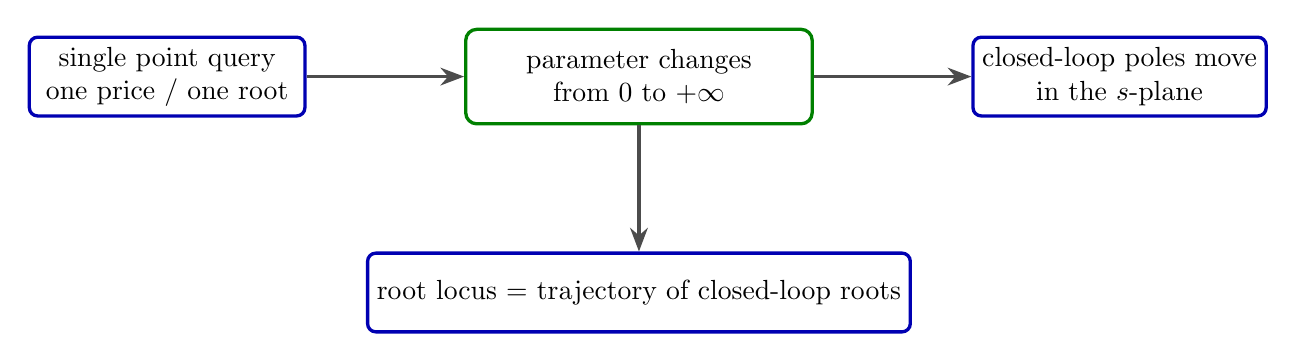
\begin{tikzpicture}[node distance=1.0cm and 1.3cm]
  \node[card] (a) {single point query\\one price / one root};
  \node[center, right=2.0cm of a] (b) {parameter changes\\from $0$ to $+\infty$};
  \node[card, right=2.0cm of b] (c) {closed-loop poles move\\in the $s$-plane};
  \node[card, below=1.6cm of b] (d) {root locus = trajectory of closed-loop roots};

  \draw[flow] (a) -- (b);
  \draw[flow] (b) -- (c);
  \draw[flow] (b) -- (d);
\end{tikzpicture}
\end{document}
